\chapter{Reproducibility and artifact evaluation}
\label{ch:repro}

How much of computational science can actually be re-run? It is an uncomfortable question, and the
honest answers are sobering --- which is why our community has built a process to force the issue:
\emph{artifact evaluation}, now standard at computer-science conferences, checks that the software
behind a paper actually exists, runs, and supports its claims. It is the sharpest test of
everything this note has argued for, and it turns out that Software Heritage answers its central
need almost perfectly. \textsc{ardc}, in other words, was the preparation; this chapter is the exam.

\takeaway{Artifact evaluation is the question this whole note was answering.}

\section{The reproducibility crisis}

The motivation is uncomfortable. When Collberg and Proebsting went looking for the code behind
several hundred papers from top computer-systems conferences, they found that, for a large majority,
the code could not be obtained, or could not be built~\autocite{Collberg2016}. Not refuted ---
simply \emph{unavailable}, or unbuildable, and so impossible to check at all. You cannot reproduce
what you cannot run; and, as the free-software tradition has always insisted, you cannot truly
inspect what you cannot read. A result resting on code is only as solid as our ability to get
\emph{that} code, at \emph{that} version, and run it again --- the gold standard being a
\emph{reproducible build} that yields, bit for bit, the same artifact from the same
source.\footnote{\url{https://reproducible-builds.org/}} The whole apparatus of artifact evaluation
exists to push back against this state of affairs.

\section{Artifact evaluation and badging}

Artifact evaluation began, fittingly, as a contest: at ESEC/FSE 2011, where the first prize went to
Vouillon and Di Cosmo. What started as an experiment is now a near-universal standard, codified by
the ACM \emph{Artifact Review and Badging} policy~\autocite{acmbadging}, which defines three
independent families of badge (Figure~\ref{fig:badges}):

\begin{description}[leftmargin=!,labelwidth=3.6cm,font=\bfseries\sffamily]
  \item[Artifacts Available] the artifacts are placed in a publicly accessible archival repository,
        with a unique identifier.
  \item[Artifacts Evaluated] the artifacts are documented, consistent, complete, and exercisable
        (\emph{Functional}) --- and, a notch higher, structured carefully for reuse
        (\emph{Reusable}).
  \item[Results Reproduced] the paper's results were independently obtained by others, with the
        authors' artifacts (\emph{Reproduced}) or without them (\emph{Replicated}).
\end{description}

\begin{figure}[htbp]
  \centering
  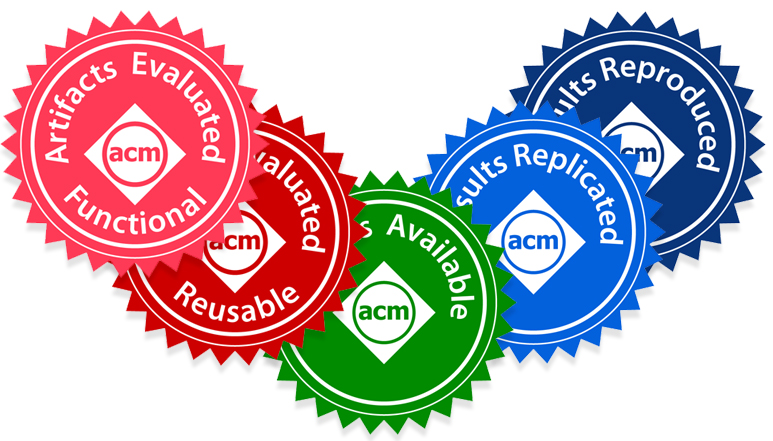
\includegraphics[width=.68\linewidth]{figures/acm-artifact-badges.png}
  \caption[The ACM artifact badges]{The ACM \emph{Artifact Review and Badging} badges. The
  \emph{Artifacts Available} badge --- a public archival repository plus a unique identifier --- is
  the one Software Heritage satisfies most literally.}
  \label{fig:badges}
\end{figure}

The practice has swept the field --- programming languages, software engineering, systems, security,
databases, high-performance computing --- to the point of routine: at EuroSys 2025 some 93\% of
papers earned the \emph{Functional} badge, and nearly half pursued \emph{Results Reproduced}. And it
is spreading beyond computer science: the AEA Data Editor now mandates a code-and-data audit for the
economics journals, initiatives such as CodeCheck and ReScience C independently re-run published
code, and NISO has generalised the whole badging scheme across the sciences~\autocite{nisorp31}.

\section{Artifact evaluation with Software Heritage}

Look again at the first badge. \emph{Artifacts Available} asks for two things: a publicly accessible
archival repository, and a unique identifier for the object. For decades this has been met by the
legacy recipe --- a zip deposited on Zenodo, figshare, or in the ACM Digital Library, with a DOI. We
have already seen, at length, why that recipe is weak for \emph{source code}: a DOI certifies a
landing page rather than the bytes (Chapter~\ref{ch:identifiers}); the deposit can change, carries no
granularity, and discards the development history (Chapter~\ref{ch:foundations}). Everything the
badge really wants --- a durable archive and a unique, verifiable name --- is exactly what
\textsc{ardc} delivers: archive the living repository in Software Heritage, and reference it with a
\textsc{swhid}.

This is not a departure from policy; it is the rigorous way to follow it. Software Heritage is
already among the archives ACM accepts for the \emph{Available} badge, the \textsc{swhid} is now
ISO/IEC 18670, and the software-engineering community has explicitly asked that it be used for
artifact evaluation~\autocite{sigsoftaecsoftware2022,isoiec18670}. The gain is sharpest for the
\emph{reviewer}. A DOI gives a reviewer a link to follow and a record to trust; a \textsc{swhid}
gives something a DOI never can --- the ability to \emph{recompute the identifier from the bytes
under review and check that it matches}, offline, in under a minute. If it matches, the reviewer
holds cryptographic proof that the artifact in hand is exactly the artifact the authors named. If it
does not, that too is a finding.

\begin{handson}[Hands-on: verify an artifact as a reviewer]
You are handed an artifact and the \textsc{swhid} the authors published for it.
\begin{enumerate}[nosep,leftmargin=*]
  \item Verify a file against its claimed content \textsc{swhid}: \texttt{swhid verify file.c
        swh:1:cnt:<hex>} --- it exits 0 only if the bytes match (Appendix~\ref{app:swhid-tools}).
  \item Re-compute the directory \textsc{swhid} of the whole artifact tree and compare it with the
        one in the paper. No archive, no network, and no trust required.
\end{enumerate}
\end{handson}

For the \emph{organiser}, the move is equally small: name Software Heritage in the call for
artifacts, and ask authors to put the qualified \textsc{swhid} of the precise artifact in the paper.
Each badge then maps cleanly onto a SWH-native check:

\begin{table}[htbp]
  \centering\small
  \begin{tabularx}{\linewidth}{@{}lX@{}}
    \toprule
    \textbf{ACM badge} & \textbf{Software Heritage--native check} \\
    \midrule
    Artifacts Available     & archived in Software Heritage; a qualified \textsc{swhid} in the paper \\
    Evaluated --- Functional & the reviewer fetches the \emph{exact} SWHID-pinned tree; no ``which zip?'' \\
    Evaluated --- Reusable   & \texttt{codemeta.json} + \texttt{CITATION.cff} + an \textsc{spdx} licence, under that \textsc{swhid} \\
    Results Reproduced      & reproduction starts from a verifiable, immutable identifier \\
    \bottomrule
  \end{tabularx}
  \caption[Badges mapped to SWH checks]{Each ACM badge mapped onto its Software Heritage--native check.}
  \label{tab:badge-crosswalk}
\end{table}

\takeaway{A reviewer can verify a \textsc{swhid} offline in a minute --- a DOI offers nothing of the
kind.}

\section{Double-blind review, and dense pinpointing}

Artifact evaluation often happens under \emph{double-blind} review, which seems to pose a problem:
how do you share your code without revealing who wrote it? Tools that rewrite a repository's history
to anonymise it are fragile, and they leak. The intrinsic identifier sidesteps the whole difficulty.
A \emph{directory} \textsc{swhid} is computed from content alone --- no author, no origin, no commit
metadata, nothing to scrub --- and it works for any technology, not just Git. Submit the
\texttt{dir} \textsc{swhid}; reviewers confirm the bytes are exactly yours while learning nothing
about you.

The same idea scales to a paper that pinpoints code throughout its body. Modern papers already do
this densely: \emph{Source Code Hotspots} ties its findings to exact passages, naming each with a
qualified \textsc{swhid} so a reader can open the precise lines in the
archive~\autocite{spinellis2026hotspots}. And the part that carries \emph{provenance} is precisely
the qualifiers --- \texttt{origin}, \texttt{visit}, \texttt{anchor} --- while the core hash, the
identifier proper, reveals nothing about authorship. So the \emph{only} difference between the double-blind
submission and the camera-ready version is removing, then restoring, those qualifiers: the core
hashes are identical, and every pinpoint a reviewer checked during blind review stays valid, to the
character, in the final paper. One mechanical, fully reversible edit --- no history-rewriting, no
risk of a leak.

\takeaway{Double-blind vs camera-ready: strip, then restore, the qualifiers --- the content hash
never changes.}

\begin{handson}[Hands-on: a double-blind artifact]
Compute the directory \textsc{swhid} of your artifact tree (\texttt{swhid dir ./}; see
Appendix~\ref{app:swhid-tools}) and submit \emph{that}. It names your exact bytes and nothing else.
After acceptance, archive the repository and add the \texttt{origin}/\texttt{anchor} qualifiers ---
the same identifier, now pointing home.
\end{handson}

\section{Built into the record of science}

Best of all is when none of this is left to the author's goodwill. Since November 2020 the journal
\emph{eLife} has archived the code behind every article in Software Heritage automatically, embedding
the \textsc{swhid} in the article's machine-readable metadata and validating it before
publication~\autocite{elifeswh2020}. Availability stops being a promise a reviewer checks once, and
becomes a durable property of the published record itself --- which is, in the end, exactly where it
belongs.

That is the case for building artifact evaluation on Software Heritage. What remains is to look
outward: at how widely this is already being adopted, the policy that now backs it, and the larger
mission it serves. That is the final chapter.
